\documentclass[12pt]{article}

\usepackage[utf8]{inputenc}
\usepackage{listings}
\usepackage{fancyvrb}
\usepackage{geometry}
\usepackage{color}
\usepackage{xcolor}
\usepackage{todonotes}
\usepackage{graphicx}
\usepackage[]{acronym}
\usepackage{float}
\usepackage[parfill]{parskip}
\usepackage{csquotes}
\usepackage{pgffor} % Loops
% \usepackage[section]{placeins} % ensure that figures appear in the section they're associated with
\usepackage{mathtools}
\usepackage[backend=biber]{biblatex}
\usepackage[american]{babel}
\usepackage{hyperref}

\addbibresource{bib.bib}

% Code listing setup:
% https://tex.stackexchange.com/a/83100/105226
\colorlet{punct}{red!60!black}
\definecolor{background}{HTML}{EEEEEE}
\definecolor{delim}{RGB}{20,105,176}
\colorlet{numb}{magenta!60!black}
\lstdefinelanguage{json}{
	literate=
	*{0}{{{\color{numb}0}}}{1}
	{1}{{{\color{numb}1}}}{1}
	{2}{{{\color{numb}2}}}{1}
	{3}{{{\color{numb}3}}}{1}
	{4}{{{\color{numb}4}}}{1}
	{5}{{{\color{numb}5}}}{1}
	{6}{{{\color{numb}6}}}{1}
	{7}{{{\color{numb}7}}}{1}
	{8}{{{\color{numb}8}}}{1}
	{9}{{{\color{numb}9}}}{1}
	{:}{{{\color{punct}{:}}}}{1}
	{,}{{{\color{punct}{,}}}}{1}
	{\{}{{{\color{delim}{\{}}}}{1}
	{\}}{{{\color{delim}{\}}}}}{1}
	{[}{{{\color{delim}{[}}}}{1}
	{]}{{{\color{delim}{]}}}}{1},
}
\lstset{ 
	language=Python, % choose the language of the code
	basicstyle=\fontfamily{pcr}\selectfont\scriptsize,
	keywordstyle=\color{black}\bfseries, % style for keywords    
	frame=single, % adds a frame around the code
	numbers=left,
	escapechar=|
	tabsize=2, % sets default tabsize to 2 spaces
	keywordstyle=\color{blue},
	stringstyle=\color{red},
	commentstyle=\color{gray},
	morecomment=[l][\color{magenta}]{\#}
	captionpos=b, % sets the caption-position to bottom
	breaklines=true, % sets automatic line breaking
	postbreak=\mbox{\textcolor{red}{$\hookrightarrow$}\space},
	breakatwhitespace=false,
}

\begin{document}
	
\title{Computer Algorithms -- Project report: Pathfinding with A*}
\author{Saleh Shehata \& Dennis Weber}
\maketitle

\begin{abstract}
	\todo[inline]{ABSTRACT HERE}
\end{abstract}

\section*{Abbreviations}
\begin{acronym}[SIFT]
	\setlength{\parskip}{0ex}
	\setlength{\itemsep}{1ex}
	\acro{DoG}{Difference of Gaussian}
	\acro{SIFT}{Scale Invariant Feature Transform}	
\end{acronym}

\section{Introduction}
\todo[inline]{TODO}

\section{Description of A*}
A* is a extension to Dijkstra's pathfinding algorithm\cite{Dijkstra1959}, in that A* adds a \enquote{heuristic} to prefer nodes which are more likely to be those who actually lie on the path to the target node.

As part of this project, we implement A* in the programming language \textit{python}. This section contains the source code and explanations how it works.
The complete code can be found in the appendix \ref{sec:pythonCode} or on GitHub.
\footnote{\url{https://github.com/Nijin22/pythonAStar}}
The basis for our implementation is the paper by Hart, Nilsson and Raphael\cite{hartNilssonRaphael} in combination with the pseudocode section on the A* Wikipedia page.\cite{wiki:astar}

\subsection{Input File}
Our script is designed, so that the pathfinding problem can be read in as a \texttt{json} file.

It contains a list of \textit{nodes}, which can represent navigational points in the problem.
(E.g. Crossings, highway entrances, subway stations, \ldots)
For each node, the geographical position is also stored (in \texttt{x} and \texttt{y} attributes).
These can later be used as input to the heuristic.

Additionally, there also is a list of \textit{edges}, which are used to represent connections between the nodes.
(E.g. streets, walkways, highways, subway tracks, \ldots)
Each edge has a associated cost, representing the amount of \enquote{effort} (e.g. time required, fuel spent, \ldots) which needs to be spent to move from the \texttt{start} to the \texttt{end} node.

Finally, the \texttt{startNode} and \texttt{targetNode} define between which nodes a path shall be searched for.
\lstinputlisting[language=json]{../exampleProblem.json}

\subsection{Code Description}
To explain how the algorithm works, we use the example problem displayed in figure \ref{fig:ex1}.
In this problem, the goal is to move from node \texttt{A} to \texttt{E}.
\begin{figure}[H]
	\centering
	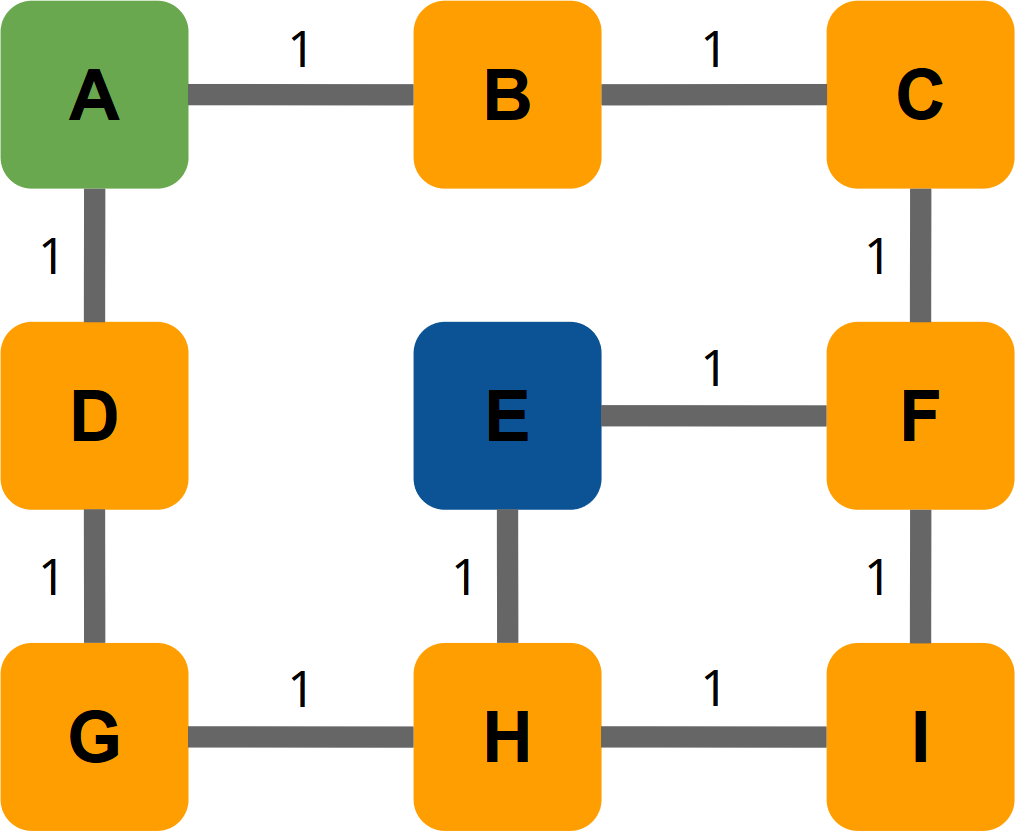
\includegraphics[width=0.7\linewidth]{sources/ex1}
	\caption{The example problem}
	\label{fig:ex1}
\end{figure}


In the beginning relevant python packages are loaded into the script.
\begin{itemize}
	\item \texttt{sys} is used, as it provides access to the \texttt{argv} array, which is filled with program parameters. This allows our script to accept problem files with different file names or locations
	\item \texttt{math} provides access to certain math operations, like \texttt{math.sqrt()} to calculate the square root of a number.
	\item \texttt{json} allows the parsing of a \texttt{json} file, which is used to define the problem.
	\item \texttt{networkx} is a graph library.\footnote{\url{https://networkx.github.io/documentation/stable/tutorial.html}} It is used to store and perform operations on the problem graph.
\end{itemize}
\begin{lstlisting}
import sys
import math
import json
import networkx as nx
\end{lstlisting}

As the next step, the program parameters are checked for a possible overwrite of the problem file name, or the program defaults into \texttt{exampleProblem.json}.
This json file is then read and the nodes and edges are added to a directed graph.

\begin{lstlisting}
# Step 1: Read input into graph
if (len(sys.argv) > 1) and (sys.argv[1] != ""):
	inputfile = sys.argv[1]
else:
	inputfile = "exampleProblem.json"
graph = nx.DiGraph()
startNode = ''
targetNode = ''
with open(inputfile) as f:
	problem = json.loads(f.read())
	for node in problem['nodes']:
	graph.add_node(node['id'], x=node['X'], y=node['Y'])
	for edge in problem['edges']:
	graph.add_edge(edge['start'], edge['end'], cost=edge['cost'])
	startNode = problem['startNode']
	targetNode = problem['targetNode']
	f.close()
\end{lstlisting}

Now two sets of nodes are initialized.
The first set, \texttt{checkedNodes} will contain nodes for which the algorithm will already have performed all operations.
This set is empty in the beginning.
The other set, \texttt{toCheckNodes} -- often also referred to as \enquote{open set} -- will contain all candidates which could contribute to a valid path.
In the beginning, this is only the node from which the search will start.
\begin{lstlisting}
checkedNodes = set()
toCheckNodes = set(startNode) # Begin with the start node
\end{lstlisting}
Additionally, each node in the graph will be supplied with values for \texttt{costToReach}, which represents the current costs to reach this node (if such a way has been found) and a \texttt{heuristic}, which will be explained in a later section.
Since the search starts at the start node, the \texttt{costToReach} value of it is set to 0.
\begin{lstlisting}
graph.nodes[startNode]['costToReach'] = 0 # cost to reach start Node is 0.
graph.nodes[startNode]['heuristic'] = calcHeuristic(startNode, targetNode)
\end{lstlisting}

\section{Alternative Heuristics}
\todo[inline]{Saleh will do this part}


\printbibliography

%%%%%%%%%%%%%%%%%%%%%%%%%%%%
% Appendix
%%%%%%%%%%%%%%%%%%%%%%%%%%%%
\newgeometry{left=1cm, right=1cm, bottom=3cm, top=1cm, onecolumn}
\section{Appendix}
\subsection{Python code}
\label{sec:pythonCode}
\lstinputlisting{../aStar.py}



\end{document}